\documentclass[12pt,a4paper]{article}
\usepackage[utf8]{inputenc}
\usepackage[margin=1in]{geometry}
\usepackage{graphicx}
\usepackage{xcolor}
\usepackage{listings}
\usepackage{tcolorbox}
\usepackage{hyperref}
\usepackage{tikz}
\usepackage{amssymb}
\usepackage{enumitem}
\usepackage{fancyhdr}

% Page styling
\pagestyle{fancy}
\fancyhf{}
\rhead{JavaFX Gaming E-Commerce}
\lhead{\textcolor{purple}{\textbf{ShopEase}}}
\cfoot{\thepage}

% Define colors
\definecolor{codebackground}{RGB}{248,249,250}
\definecolor{purple}{RGB}{102,126,234}
\definecolor{pink}{RGB}{118,75,162}
\definecolor{green}{RGB}{40,167,69}
\definecolor{red}{RGB}{220,53,69}
\definecolor{blue}{RGB}{23,162,184}
\definecolor{yellow}{RGB}{255,193,7}

% Code listing style
\lstset{
    backgroundcolor=\color{codebackground},
    basicstyle=\ttfamily\small,
    breaklines=true,
    captionpos=b,
    commentstyle=\color{green!60!black},
    keywordstyle=\color{purple}\bfseries,
    numbers=left,
    numberstyle=\tiny\color{gray},
    stringstyle=\color{red!60!black},
    frame=single,
    rulecolor=\color{gray!30},
    showstringspaces=false,
    tabsize=4,
    language=Java,
    morekeywords={var, record}
}

% Fun colored boxes
\newtcolorbox{funbox}[1]{
    colback=#1!5!white,
    colframe=#1!75!black,
    fonttitle=\bfseries,
    rounded corners
}

\newtcolorbox{analogybox}{
    colback=yellow!10,
    colframe=yellow!80!black,
    title=\textbf{🧠 Real-Life Analogy},
    fonttitle=\bfseries,
    rounded corners,
    enhanced
}

\newtcolorbox{summarybox}{
    colback=green!10,
    colframe=green!70!black,
    title=\textbf{✨ Mini Summary},
    fonttitle=\bfseries,
    rounded corners
}

\hypersetup{
    colorlinks=true,
    linkcolor=purple,
    filecolor=purple,
    urlcolor=blue,
}

\begin{document}

% =====================================================
% TITLE PAGE
% =====================================================
\begin{titlepage}
    \centering
    \vspace*{2cm}

    {\Huge\bfseries\textcolor{purple}{🎮 ShopEase Gaming Store 🎮}\par}
    \vspace{0.5cm}
    {\Large\textit{A JavaFX E-Commerce Adventure}}\par
    \vspace{2cm}

    {\LARGE\textbf{Hamdan Yasser}}\par
    \vspace{1cm}

    \begin{tcolorbox}[colback=purple!15, colframe=purple!75!black, width=0.8\textwidth, arc=10pt]
        \centering
        {\Large\textit{``Your one-stop shop for all things gaming –}}\\
        {\Large\textit{built with pure Java code, no FXML magic!''}}
    \end{tcolorbox}

    \vspace{2cm}

    {\large \textcolor{gray}{JavaFX 21 | MySQL | JWT Authentication | Pure Java UI}}\par

    \vfill

    {\large \today}\par
\end{titlepage}

\tableofcontents
\newpage

% =====================================================
% OVERVIEW
% =====================================================
\section{✨ Simple Overview}

\begin{funbox}{purple}
\subsection*{What Does This Project Do? 🤔}

Imagine you're building your own online gaming store – like Amazon, but cooler and specifically for gamers! This project is a \textbf{complete e-commerce application} where:

\begin{itemize}[leftmargin=*]
    \item 🛒 Customers can \textbf{browse} thousands of games, consoles, and accessories
    \item 🔍 They can \textbf{filter} by platform (PS5, Xbox, Nintendo Switch, PC, Steam Deck...)
    \item 🎯 Search by genre (Action, RPG, Horror, Sports...)
    \item ⭐ Read and write \textbf{reviews}
    \item 💳 Add items to cart and \textbf{checkout}
    \item 📦 Track their \textbf{orders}
    \item ♡ Save favorites to a \textbf{wishlist}
    \item 💎 Earn \textbf{loyalty points} with every purchase
    \item 👨‍💼 Admins can manage products, orders, and promotions
\end{itemize}

\textbf{All of this} is built using JavaFX – and here's the kicker: \textbf{NO FXML files!} Everything is created programmatically using pure Java code.

\end{funbox}

\begin{analogybox}
\textbf{Think of this app like a digital shopping mall:}

\begin{itemize}[leftmargin=*]
    \item The \textbf{Controllers} are like the different stores (Electronics Store, Checkout Counter, Customer Service Desk)
    \item The \textbf{Models} are like the products on the shelves
    \item The \textbf{Services} are like the store managers who handle complex operations
    \item The \textbf{DAOs} are like the warehouse workers who fetch stuff from the database
    \item The \textbf{Security} layer is like the security guards checking IDs
    \item The \textbf{Database} is the giant warehouse in the back
\end{itemize}

When you (the customer) want to buy a game, you walk through the mall (navigate screens), pick items (add to cart), go to checkout (pay), and the warehouse ships it to you!
\end{analogybox}

\newpage

% =====================================================
% APP STARTUP
% =====================================================
\section{🚀 How the App Starts}

\subsection{The Magic Beginning}

Every JavaFX app needs a special class that extends \texttt{Application}. Think of it as the \textbf{power button} of your app!

\subsection*{📦 HelloApplication.java}

\begin{analogybox}
This class is like the \textbf{receptionist of a hotel}. When you arrive, the receptionist:
\begin{enumerate}
    \item Opens the door (initializes the window)
    \item Shows you to your room (loads the login screen)
    \item Helps you navigate between rooms (switches between screens)
\end{enumerate}
\end{analogybox}

\subsubsection*{📦 Code Snippet 1: The Main Method}

\begin{lstlisting}
public static void main(String[] args) {
    launch();
}
\end{lstlisting}

\textbf{Explanation:} This is where everything begins! When you run your app, Java calls this \texttt{main} method. The \texttt{launch()} method is a special JavaFX command that says \textit{``Hey, start the JavaFX application!''} It's like pressing the START button on your PlayStation.

\subsubsection*{📦 Code Snippet 2: The start() Method}

\begin{lstlisting}
@Override
public void start(Stage stage) throws Exception {
    mainStage = stage;
    setRoot(new LoginController());
    stage.setTitle("E-Commerce App");
    stage.show();
}
\end{lstlisting}

\textbf{Explanation:}
\begin{itemize}
    \item \textbf{Stage} = Think of this as the window frame. It's the container for everything!
    \item \textbf{setRoot(new LoginController())} = We're telling the app: \textit{``Show the login screen first!''}
    \item \textbf{stage.setTitle(...)} = Sets the window title (what you see at the top)
    \item \textbf{stage.show()} = Actually displays the window on screen!
\end{itemize}

\subsubsection*{📦 Code Snippet 3: The Screen Switcher}

\begin{lstlisting}
public static void setRoot(Object controller) {
    try {
        Parent root = null;

        if (controller instanceof LoginController) {
            root = ((LoginController) controller).createView();
        } else if (controller instanceof CustomerHomeController) {
            root = ((CustomerHomeController) controller).createView();
        } else if (controller instanceof CartController) {
            root = ((CartController) controller).createView();
        }
        // ... more screens ...

        if (root != null) {
            Scene scene = new Scene(root);
            ToastNotification.initialize(scene);
            mainStage.setScene(scene);
            mainStage.centerOnScreen();
        }
    } catch (Exception e) {
        e.printStackTrace();
    }
}
\end{lstlisting}

\textbf{Explanation:} This is the \textbf{magic navigation system}! Imagine it like a GPS:
\begin{itemize}
    \item You give it a destination (controller)
    \item It checks \textit{``Which screen do you want?''}
    \item Calls the \texttt{createView()} method to build that screen
    \item Wraps it in a Scene (the content holder)
    \item Shows it on the Stage (the window)
    \item Centers it on your screen so it looks nice!
\end{itemize}

\begin{summarybox}
\textbf{In short:} HelloApplication is the boss! It starts the app, loads the login screen, and provides a way to switch between different screens. Whenever you want to go from Login → Home → Cart, you call \texttt{HelloApplication.setRoot(new SomeController())}!
\end{summarybox}

\newpage

% =====================================================
% PROJECT STRUCTURE
% =====================================================
\section{📂 Project Structure Explained}

Your project is organized like a well-sorted closet! Let me break it down:

\begin{center}
\begin{tikzpicture}[
    every node/.style={font=\small},
    level 1/.style={sibling distance=3cm, level distance=1.5cm},
    level 2/.style={sibling distance=2cm, level distance=1.2cm}
]
\node[draw, fill=purple!20, rounded corners, font=\bfseries] {FinalProject}
    child {node[draw, fill=green!20, rounded corners] {📦 model}}
    child {node[draw, fill=blue!20, rounded corners] {🎮 controller}}
    child {node[draw, fill=yellow!20, rounded corners] {⚙️ service}}
    child {node[draw, fill=red!20, rounded corners] {🗄️ dao}}
    child {node[draw, fill=pink!20, rounded corners] {🔒 security}};
\end{tikzpicture}
\end{center}

\subsection{🏗️ Folder Breakdown}

\begin{tcolorbox}[colback=green!10, colframe=green!70!black, title=\textbf{📦 model}, fonttitle=\bfseries]
\textbf{What's inside:} All your data classes (User, Product, Order, Review, etc.)

\textbf{Analogy:} These are like the \textbf{blueprint cards} for your products. If you're selling a PlayStation 5, the Product model is the card that says: \textit{``Name: PS5, Price: \$499, Stock: 10''}

\textbf{Examples:}
\begin{itemize}
    \item \texttt{User.java} – Represents a customer or admin
    \item \texttt{Product.java} – Represents a game, console, or accessory
    \item \texttt{Order.java} – Represents a customer's order
    \item \texttt{ShoppingCart.java} – Your shopping cart data
\end{itemize}
\end{tcolorbox}

\begin{tcolorbox}[colback=blue!10, colframe=blue!70!black, title=\textbf{🎮 controller}, fonttitle=\bfseries]
\textbf{What's inside:} All your UI screens (Login, Register, Home, Cart, Checkout...)

\textbf{Analogy:} Controllers are like \textbf{different rooms in your house}. The LoginController is the front door, CustomerHomeController is the living room, CartController is the kitchen where you prepare your order!

\textbf{Examples:}
\begin{itemize}
    \item \texttt{LoginController.java} – The login screen
    \item \texttt{CustomerHomeController.java} – Main shopping page
    \item \texttt{CartController.java} – Shopping cart page
    \item \texttt{AdminProductsController.java} – Admin panel
\end{itemize}
\end{tcolorbox}

\begin{tcolorbox}[colback=yellow!10, colframe=yellow!70!black, title=\textbf{⚙️ service}, fonttitle=\bfseries]
\textbf{What's inside:} Business logic – the smart helpers!

\textbf{Analogy:} Services are like the \textbf{store managers}. They handle complex tasks like \textit{``Register this new user,''} \textit{``Calculate the loyalty points,''} or \textit{``Send a welcome email.''}

\textbf{Examples:}
\begin{itemize}
    \item \texttt{AuthService.java} – Handles login and registration
    \item \texttt{CartService.java} – Manages shopping cart operations
    \item \texttt{OrderService.java} – Processes orders
    \item \texttt{LoyaltyService.java} – Manages loyalty points
\end{itemize}
\end{tcolorbox}

\begin{tcolorbox}[colback=red!10, colframe=red!70!black, title=\textbf{🗄️ dao}, fonttitle=\bfseries]
\textbf{What's inside:} Database access objects – the data fetchers!

\textbf{Analogy:} DAOs are like \textbf{warehouse workers}. When you need a product from the database, the DAO goes into the warehouse (database), finds it, and brings it back to you.

\textbf{Examples:}
\begin{itemize}
    \item \texttt{UserDao.java} – Fetches/saves users from database
    \item \texttt{ProductDao.java} – Fetches/saves products
    \item \texttt{OrderDao.java} – Fetches/saves orders
    \item \texttt{DBConnection.java} – The bridge to the database
\end{itemize}
\end{tcolorbox}

\begin{tcolorbox}[colback=pink!10, colframe=pink!70!black, title=\textbf{🔒 security}, fonttitle=\bfseries]
\textbf{What's inside:} Authentication and security features

\textbf{Analogy:} Security is like the \textbf{bouncers at a nightclub}. They check your ID (JWT token), make sure your password is correct (bcrypt hashing), and only let authorized people in!

\textbf{Examples:}
\begin{itemize}
    \item \texttt{Session.java} – Keeps track of who's logged in
    \item \texttt{JwtService.java} – Creates and verifies JWT tokens
    \item \texttt{PasswordHasher.java} – Encrypts passwords
    \item \texttt{AuthGuard.java} – Blocks unauthorized access
\end{itemize}
\end{tcolorbox}

\newpage

% =====================================================
% MODELS
% =====================================================
\section{📦 Model Classes (The Data Blueprints)}

\subsection{🧩 User.java}

\textbf{What it does:} Represents a person using the app (customer or admin).

\begin{analogybox}
Think of User like a \textbf{membership card} at Costco. It has your name, email, address, and tells the store if you're a regular member or a staff member (role).
\end{analogybox}

\subsubsection*{📦 Code Snippet 1: The Fields}

\begin{lstlisting}
public class User {
    private int id;
    private String name;
    private String email;
    private String passwordHash;
    private String role;  // "CUSTOMER" or "ADMIN"
    private String address;

    // ... constructors and getters/setters ...
}
\end{lstlisting}

\textbf{Explanation:}
\begin{itemize}
    \item \textbf{id} = A unique number for this user (like a student ID)
    \item \textbf{name} = The person's full name
    \item \textbf{email} = Their email address (used for login)
    \item \textbf{passwordHash} = Their password (encrypted for security!)
    \item \textbf{role} = Either ``CUSTOMER'' or ``ADMIN''
    \item \textbf{address} = Where to ship their orders
\end{itemize}

\begin{summarybox}
\textbf{In short:} User is a simple data container. It holds all the information about a person. No fancy logic – just pure data!
\end{summarybox}

\newpage

\subsection{🧩 Product.java}

\textbf{What it does:} Represents a product in your store (game, console, accessory).

\begin{analogybox}
Product is like a \textbf{sticker on a box at Best Buy}. The sticker tells you the name, price, category, how many are in stock, and what platforms it works with!
\end{analogybox}

\subsubsection*{📦 Code Snippet 1: The Main Fields}

\begin{lstlisting}
public class Product {
    private int id;
    private String name;
    private String category;  // "Console", "Game", "Accessory"
    private double price;
    private String description;
    private String imagePath;
    private int stock;
    private double discount;  // percentage (0-100)
    private List<String> platforms;  // ["PS5", "Xbox", "PC"]
    private List<String> genres;     // ["Action", "RPG"]
    private String ageRating;        // "E", "T", "M", etc.
    private String productType;      // "Physical", "Digital", "GiftCard"

    // ...
}
\end{lstlisting}

\textbf{Explanation:}
\begin{itemize}
    \item \textbf{id} = Unique product ID
    \item \textbf{name} = Product name (e.g., ``PlayStation 5'')
    \item \textbf{category} = Type of product (Console, Game, Accessory)
    \item \textbf{price} = How much it costs
    \item \textbf{stock} = How many are available
    \item \textbf{discount} = Sale percentage (15 = 15\% off)
    \item \textbf{platforms} = What gaming systems it works on
    \item \textbf{genres} = Game genres (if it's a game)
    \item \textbf{productType} = Physical (shipped), Digital (code), or GiftCard
\end{itemize}

\subsubsection*{📦 Code Snippet 2: Helper Methods}

\begin{lstlisting}
public double getEffectivePrice() {
    return price * (1 - (discount / 100.0));
}

public boolean isDigital() {
    return "Digital".equals(productType) || "GiftCard".equals(productType);
}

public String getPlatformsAsString() {
    if (platforms == null || platforms.isEmpty()) {
        return "N/A";
    }
    return String.join(", ", platforms);
}
\end{lstlisting}

\textbf{Explanation:}
\begin{itemize}
    \item \textbf{getEffectivePrice()} = Calculates the final price after discount
    \item \textbf{isDigital()} = Checks if this product is digital (no shipping needed)
    \item \textbf{getPlatformsAsString()} = Converts the list to ``PS5, Xbox, PC''
\end{itemize}

\begin{summarybox}
\textbf{In short:} Product holds all the details about an item in your store. It has the price, stock, discounts, and helper methods to calculate the final price or check if it's digital!
\end{summarybox}

\newpage

\subsection{🧩 Order.java \& OrderItem.java}

\textbf{What they do:} When a customer buys stuff, you create an Order with multiple OrderItems inside.

\begin{analogybox}
Think of Order as a \textbf{receipt from McDonald's}:
\begin{itemize}
    \item The \textbf{Order} is the whole receipt (order number, total price, status)
    \item Each \textbf{OrderItem} is a line on the receipt (``2x Big Mac - \$5.99 each'')
\end{itemize}
\end{analogybox}

\subsubsection*{📦 Code Snippet: Order.java}

\begin{lstlisting}
public class Order {
    private int id;
    private int userId;            // Who placed this order?
    private double total;          // Total price
    private String status;         // "Pending", "Processing", "Shipped", "Delivered"
    private Timestamp createdAt;   // When was it ordered?
    private List<OrderItem> items; // What did they buy?

    // ... getters and setters ...
}
\end{lstlisting}

\subsubsection*{📦 Code Snippet: OrderItem.java}

\begin{lstlisting}
public class OrderItem {
    private int id;
    private int orderId;     // Which order does this belong to?
    private int productId;   // Which product?
    private int quantity;    // How many?
    private double price;    // Price per unit at time of purchase

    private String productName;  // For display purposes

    // ... getters and setters ...
}
\end{lstlisting}

\textbf{Explanation:}
\begin{itemize}
    \item One \textbf{Order} can have many \textbf{OrderItems}
    \item Example: Order \#42 contains 2 OrderItems: ``PS5 x1'' and ``Spider-Man x1''
    \item The \texttt{status} field tracks the order's journey: Pending → Processing → Shipped → Delivered
\end{itemize}

\begin{summarybox}
\textbf{In short:} Order = the shopping receipt. OrderItem = each line on the receipt. Together they represent a customer's purchase!
\end{summarybox}

\newpage

\subsection{🧩 ShoppingCart.java}

\textbf{What it does:} Holds the items a customer has added to their cart (before checkout).

\begin{analogybox}
ShoppingCart is like your actual \textbf{shopping cart at Target}. You throw items in (addItem), take them out (remove), check the total (getTotal), and when you're done shopping, you checkout and empty it (clear)!
\end{analogybox}

\subsubsection*{📦 Code Snippet}

\begin{lstlisting}
public class ShoppingCart {
    private static final Map<Integer, Integer> items = new HashMap<>();
    private static final Map<Integer, Double> prices = new HashMap<>();

    public static void addItem(int productId, double price, int quantity, int stock) {
        int current = items.getOrDefault(productId, 0);
        int newQty = Math.min(current + quantity, stock);
        items.put(productId, newQty);
        prices.put(productId, price);
    }

    public static double getTotal() {
        return items.entrySet().stream()
                .mapToDouble(e -> prices.get(e.getKey()) * e.getValue())
                .sum();
    }

    public static void clear() {
        items.clear();
        prices.clear();
    }
}
\end{lstlisting}

\textbf{Explanation:}
\begin{itemize}
    \item \textbf{items} = A map of (productId → quantity). Example: \{5: 2, 7: 1\} means ``2 of product 5, 1 of product 7''
    \item \textbf{prices} = A map of (productId → price)
    \item \textbf{addItem()} = Adds more items, but won't exceed stock
    \item \textbf{getTotal()} = Multiplies each item's price by quantity and sums it all up
    \item \textbf{clear()} = Empties the cart (after checkout)
\end{itemize}

\begin{summarybox}
\textbf{In short:} ShoppingCart is a temporary storage for items before the customer buys them. It's like a digital shopping basket!
\end{summarybox}

\newpage

\subsection{🧩 Review.java}

\textbf{What it does:} Represents a customer's review of a product.

\begin{analogybox}
Review is like a \textbf{Yelp review} for a restaurant. It has a star rating (1-5), a comment (``This game was amazing!''), and shows who wrote it and when.
\end{analogybox}

\subsubsection*{📦 Code Snippet}

\begin{lstlisting}
public class Review {
    private int id;
    private int productId;    // Which product is being reviewed?
    private int userId;       // Who wrote the review?
    private int rating;       // 1 to 5 stars
    private String comment;   // "Amazing game! Loved it!"
    private Timestamp createdAt;

    // Additional fields for display
    private String username;
    private String productName;

    // ... getters and setters ...
}
\end{lstlisting}

\textbf{Explanation:}
\begin{itemize}
    \item \textbf{rating} = 1 to 5 stars
    \item \textbf{comment} = Customer's written feedback
    \item \textbf{username} and \textbf{productName} = Extra fields added when displaying reviews (not stored in DB, but joined from other tables)
\end{itemize}

\begin{summarybox}
\textbf{In short:} Review = customer feedback. It lets users share their opinion about a product with a rating and comment!
\end{summarybox}

\newpage

\subsection{🧩 Platform.java \& Genre.java}

\textbf{What they do:} Represent gaming platforms and genres.

\begin{analogybox}
\textbf{Platform} is like the operating system tags on an app store: ``Works on iOS, Android, Windows''

\textbf{Genre} is like Netflix categories: ``Action, Comedy, Horror''
\end{analogybox}

\subsubsection*{📦 Code Snippet: Platform.java}

\begin{lstlisting}
public class Platform {
    private int id;
    private String name;           // "PlayStation 5"
    private String type;           // "Console"
    private String manufacturer;   // "Sony"
    private String iconPath;

    @Override
    public String toString() {
        return name;
    }
}
\end{lstlisting}

\subsubsection*{📦 Code Snippet: Genre.java}

\begin{lstlisting}
public class Genre {
    private int id;
    private String name;        // "Action"
    private String description; // "Fast-paced combat games"
    private String iconPath;

    @Override
    public String toString() {
        return name;
    }
}
\end{lstlisting}

\textbf{Explanation:}
\begin{itemize}
    \item These are simple reference data (like a lookup table)
    \item Products can have multiple platforms (e.g., a game works on both PS5 and Xbox)
    \item Products can have multiple genres (e.g., an Action-RPG game)
\end{itemize}

\begin{summarybox}
\textbf{In short:} Platform = gaming system tags. Genre = game category tags. They help customers filter products!
\end{summarybox}

\newpage

% =====================================================
% SECURITY
% =====================================================
\section{🔒 Security Classes (The Bouncers)}

\subsection{🧩 Session.java}

\textbf{What it does:} Keeps track of who's currently logged in.

\begin{analogybox}
Session is like your \textbf{movie ticket stub}. When you enter the theater, they give you a ticket (JWT token). Throughout the movie, you can use that ticket to prove you're allowed to be there. When you leave, you throw it away (clear).
\end{analogybox}

\subsubsection*{📦 Code Snippet}

\begin{lstlisting}
public class Session {
    private static String token;

    public static void setToken(String t) {
        token = t;
    }

    public static String getToken() {
        return token;
    }

    public static void clear() {
        token = null;
    }

    public static boolean isAuthenticated() {
        if (token == null) return false;
        boolean expiredOrInvalid = JwtService.isExpired(token);
        if (expiredOrInvalid) token = null;
        return !expiredOrInvalid;
    }

    public static int getUserId() {
        return token == null ? -1 : JwtService.getUserId(token);
    }

    public static String getUserRole() {
        return token == null ? null : JwtService.getRole(token);
    }
}
\end{lstlisting}

\textbf{Explanation:}
\begin{itemize}
    \item \textbf{token} = A static variable that stores the JWT token (one per app session)
    \item \textbf{setToken()} = Saves the token when user logs in
    \item \textbf{isAuthenticated()} = Checks if there's a valid, non-expired token
    \item \textbf{getUserId()} = Extracts the user ID from the token
    \item \textbf{clear()} = Logs the user out by deleting the token
\end{itemize}

\begin{summarybox}
\textbf{In short:} Session is like a global variable that remembers ``Who is logged in right now?'' It stores the JWT token and provides helper methods to check authentication!
\end{summarybox}

\newpage

\subsection{🧩 JwtService.java}

\textbf{What it does:} Creates and verifies JWT tokens.

\begin{analogybox}
JwtService is like a \textbf{passport office}:
\begin{itemize}
    \item \texttt{issueToken()} = Creates a new passport with your info (userId, role, email)
    \item \texttt{verify()} = Checks if a passport is real or fake
    \item \texttt{isExpired()} = Checks if the passport has expired
    \item \texttt{getUserId()} = Reads the ID from the passport
\end{itemize}
\end{analogybox}

\subsubsection*{📦 Code Snippet 1: Issue a Token}

\begin{lstlisting}
private static final String SECRET = "your-secret-key";
private static final long EXPIRATION_TIME = 1000L * 60 * 60 * 24; // 24 hours

public static String issueToken(int userId, String role, String email) {
    return JWT.create()
            .withClaim("userId", userId)
            .withClaim("role", role)
            .withClaim("email", email)
            .withIssuedAt(new Date())
            .withExpiresAt(new Date(System.currentTimeMillis() + EXPIRATION_TIME))
            .sign(Algorithm.HMAC256(SECRET));
}
\end{lstlisting}

\textbf{Explanation:}
\begin{itemize}
    \item Creates a JWT token with embedded info (userId, role, email)
    \item Sets an expiration time (24 hours from now)
    \item Signs it with a secret key so nobody can tamper with it
\end{itemize}

\subsubsection*{📦 Code Snippet 2: Verify and Extract}

\begin{lstlisting}
public static DecodedJWT verify(String token) {
    return JWT.require(Algorithm.HMAC256(SECRET))
              .build()
              .verify(token);
}

public static int getUserId(String token) {
    try {
        return verify(token).getClaim("userId").asInt();
    } catch (Exception e) {
        return -1;
    }
}

public static boolean isExpired(String token) {
    try {
        DecodedJWT jwt = verify(token);
        Date exp = jwt.getExpiresAt();
        return exp == null || exp.before(new Date());
    } catch (TokenExpiredException ex) {
        return true;
    } catch (Exception ex) {
        return true;
    }
}
\end{lstlisting}

\textbf{Explanation:}
\begin{itemize}
    \item \textbf{verify()} = Checks the token's signature is valid
    \item \textbf{getUserId()} = Extracts the userId claim from the token
    \item \textbf{isExpired()} = Checks if the token has passed its expiration date
\end{itemize}

\begin{summarybox}
\textbf{In short:} JwtService creates secure tokens when users log in, and verifies them later. It's like a passport office – issuing IDs and checking if they're legit!
\end{summarybox}

\newpage

\subsection{🧩 PasswordHasher.java}

\textbf{What it does:} Encrypts passwords using bcrypt.

\begin{analogybox}
PasswordHasher is like a \textbf{paper shredder for passwords}. You put in ``mypassword123'' and it spits out a scrambled mess like ``\$2a\$12\$Kh5...''. Even if a hacker steals the database, they can't un-shred it to see the real password!
\end{analogybox}

\subsubsection*{📦 Code Snippet}

\begin{lstlisting}
import org.mindrot.jbcrypt.BCrypt;

public class PasswordHasher {
    public static String hash(String plainPassword) {
        return BCrypt.hashpw(plainPassword, BCrypt.gensalt(12));
    }

    public static boolean verify(String plainPassword, String hashedPassword) {
        return BCrypt.checkpw(plainPassword, hashedPassword);
    }
}
\end{lstlisting}

\textbf{Explanation:}
\begin{itemize}
    \item \textbf{hash()} = Takes a plain text password (``hello123'') and scrambles it into a hashed version
    \item \textbf{gensalt(12)} = Adds extra randomness (salt) with strength 12
    \item \textbf{verify()} = Checks if a plain password matches the hashed one (used during login)
\end{itemize}

\textbf{Why bcrypt?}
\begin{itemize}
    \item \textbf{Slow by design} = Makes it hard for hackers to try millions of passwords
    \item \textbf{Salted} = Same password produces different hashes (more secure!)
    \item \textbf{One-way} = You can't reverse it to get the original password
\end{itemize}

\begin{summarybox}
\textbf{In short:} PasswordHasher is the security guard for passwords. It encrypts them when users register and verifies them when they log in. Never store plain passwords!
\end{summarybox}

\newpage

% =====================================================
% SERVICES
% =====================================================
\section{⚙️ Service Classes (The Managers)}

\subsection{🧩 AuthService.java}

\textbf{What it does:} Handles user registration and login.

\begin{analogybox}
AuthService is like the \textbf{customer service desk at a gym}:
\begin{itemize}
    \item \texttt{register()} = Sign up for a new membership
    \item \texttt{login()} = Swipe your card to enter the gym
\end{itemize}
\end{analogybox}

\subsubsection*{📦 Code Snippet 1: Register}

\begin{lstlisting}
public String register(String name, String email, String password, String address)
        throws Exception {
    // Check if email already exists
    if (userDao.findByEmail(email).isPresent()) {
        throw new Exception("Email already exists!");
    }

    // Hash the password
    String hashed = PasswordHasher.hash(password);

    // Create and save the user
    User user = new User(0, name, email, hashed, "CUSTOMER", address);
    userDao.save(user);

    // Issue a JWT token
    return JwtService.issueToken(user.getId(), user.getRole(), user.getEmail());
}
\end{lstlisting}

\textbf{Explanation:}
\begin{enumerate}
    \item Check if the email is already taken
    \item Hash the password for security
    \item Create a new User object with role = ``CUSTOMER''
    \item Save it to the database
    \item Generate a JWT token and return it (so they're auto-logged in)
\end{enumerate}

\subsubsection*{📦 Code Snippet 2: Login}

\begin{lstlisting}
public String login(String email, String password) throws Exception {
    // Find user by email
    Optional<User> optUser = userDao.findByEmail(email);
    if (optUser.isEmpty()) {
        throw new Exception("User not found!");
    }

    User user = optUser.get();

    // Verify password
    if (!PasswordHasher.verify(password, user.getPasswordHash())) {
        throw new Exception("Invalid password!");
    }

    // Issue JWT token
    return JwtService.issueToken(user.getId(), user.getRole());
}
\end{lstlisting}

\textbf{Explanation:}
\begin{enumerate}
    \item Look up the user by email
    \item If not found, throw an error
    \item Check if the password matches using bcrypt
    \item If it matches, issue a JWT token and return it
    \item If it doesn't match, throw ``Invalid password!''
\end{enumerate}

\begin{summarybox}
\textbf{In short:} AuthService is the gatekeeper. It handles signing up new users and logging them in. It talks to UserDao to save/fetch users from the database and uses PasswordHasher + JwtService for security!
\end{summarybox}

\newpage

\subsection{🧩 ProductService.java}

\textbf{What it does:} Manages products (add, update, delete, validate).

\begin{analogybox}
ProductService is like the \textbf{inventory manager at Walmart}. Before adding a product to the shelves, they make sure:
\begin{itemize}
    \item It has a valid name
    \item The price isn't negative
    \item The stock count makes sense
\end{itemize}
\end{analogybox}

\subsubsection*{📦 Code Snippet}

\begin{lstlisting}
public class ProductService {
    private final ProductDao dao = new ProductDao();

    public List<Product> getAll() {
        return dao.getAllProducts();
    }

    public void add(Product p) {
        validate(p);
        dao.insert(p);
    }

    public void update(Product p) {
        if (p.getId() <= 0)
            throw new IllegalArgumentException("Invalid product ID.");
        validate(p);
        dao.update(p);
    }

    public void delete(int id) {
        if (id <= 0)
            throw new IllegalArgumentException("Invalid ID.");
        dao.delete(id);
    }

    private void validate(Product p) {
        if (p.getName() == null || p.getName().trim().isEmpty())
            throw new IllegalArgumentException("Product name required.");
        if (p.getPrice() < 0)
            throw new IllegalArgumentException("Price cannot be negative.");
        if (p.getStock() < 0)
            throw new IllegalArgumentException("Stock cannot be negative.");
    }
}
\end{lstlisting}

\textbf{Explanation:}
\begin{itemize}
    \item \textbf{getAll()} = Fetches all products from database
    \item \textbf{add()} = Validates the product, then inserts it
    \item \textbf{update()} = Validates, then updates an existing product
    \item \textbf{delete()} = Removes a product by ID
    \item \textbf{validate()} = Business rule checks (name not empty, price/stock not negative)
\end{itemize}

\begin{summarybox}
\textbf{In short:} ProductService is the smart layer between Controllers and DAOs. It enforces business rules (validation) and delegates database work to ProductDao!
\end{summarybox}

\newpage

\subsection{🧩 CartService.java}

\textbf{What it does:} Manages the shopping cart (add items, remove, calculate total).

\begin{analogybox}
CartService is like the \textbf{shopping cart you push around in a grocery store}. You add items, remove items, and at the end, it tells you the total price!
\end{analogybox}

\subsubsection*{📦 Code Snippet}

\begin{lstlisting}
public class CartService {
    private static CartService instance;
    private final Map<Product, Integer> items = new LinkedHashMap<>();

    private CartService() {}

    public static CartService getInstance() {
        if (instance == null) instance = new CartService();
        return instance;
    }

    public void addItem(Product p, int quantity) {
        int currentQty = items.getOrDefault(p, 0);
        int newQty = Math.min(currentQty + quantity, p.getStock());
        items.put(p, newQty);
    }

    public void removeItem(Product p) {
        items.remove(p);
    }

    public void clear() {
        items.clear();
    }

    public double getTotal() {
        return items.entrySet().stream()
                .mapToDouble(e -> e.getKey().getEffectivePrice() * e.getValue())
                .sum();
    }

    public Map<Product, Integer> getItems() {
        return items;
    }
}
\end{lstlisting}

\textbf{Explanation:}
\begin{itemize}
    \item \textbf{Singleton pattern} = Only one CartService exists per app session
    \item \textbf{addItem()} = Adds products to the cart, but won't exceed stock
    \item \textbf{getTotal()} = Calculates the total price by summing up (price × quantity) for all items
    \item \textbf{clear()} = Empties the cart (after checkout)
\end{itemize}

\begin{summarybox}
\textbf{In short:} CartService is a singleton that holds the customer's shopping cart. It's like a temporary basket that exists until checkout!
\end{summarybox}

\newpage

% =====================================================
% DAOs
% =====================================================
\section{🗄️ DAO Classes (The Database Workers)}

\subsection{🧩 DBConnection.java}

\textbf{What it does:} Provides a connection to the MySQL database.

\begin{analogybox}
DBConnection is like the \textbf{Wi-Fi router in your house}. Every device (DAO) needs to connect to it to access the internet (database). When a DAO wants data, it calls \texttt{DBConnection.getInstance()} to get a connection!
\end{analogybox}

\subsubsection*{📦 Code Snippet}

\begin{lstlisting}
public class DBConnection {
    private static Properties dbProperties;

    private DBConnection() {}

    private static Properties loadDatabaseConfig() throws SQLException {
        if (dbProperties == null) {
            dbProperties = new Properties();
            try (InputStream input = DBConnection.class.getClassLoader()
                    .getResourceAsStream("db.properties")) {

                if (input == null) {
                    throw new SQLException(
                        "Unable to find db.properties file."
                    );
                }

                dbProperties.load(input);

                if (!dbProperties.containsKey("db.url") ||
                    !dbProperties.containsKey("db.username") ||
                    !dbProperties.containsKey("db.password")) {
                    throw new SQLException(
                        "db.properties is missing required fields"
                    );
                }
            } catch (IOException e) {
                throw new SQLException("Error loading database config", e);
            }
        }
        return dbProperties;
    }

    public static Connection getInstance() throws SQLException {
        try {
            Class.forName("com.mysql.cj.jdbc.Driver");

            Properties config = loadDatabaseConfig();
            String url = config.getProperty("db.url");
            String username = config.getProperty("db.username");
            String password = config.getProperty("db.password");

            return DriverManager.getConnection(url, username, password);

        } catch (ClassNotFoundException e) {
            throw new SQLException("MySQL Driver not found!", e);
        }
    }
}
\end{lstlisting}

\textbf{Explanation:}
\begin{itemize}
    \item Loads database credentials from \texttt{db.properties} file
    \item Returns a \texttt{Connection} object that DAOs use to talk to MySQL
    \item Uses JDBC (Java Database Connectivity)
\end{itemize}

\begin{summarybox}
\textbf{In short:} DBConnection is the bridge to your MySQL database. Every DAO calls it to get a connection!
\end{summarybox}

\newpage

\subsection{🧩 UserDao.java}

\textbf{What it does:} Handles all database operations for Users (find, save, update).

\begin{analogybox}
UserDao is like a \textbf{librarian} who specializes in the ``Users'' section. Need to find a user by email? Ask the UserDao. Need to save a new user? UserDao does it!
\end{analogybox}

\subsubsection*{📦 Code Snippet 1: Find User by Email}

\begin{lstlisting}
public Optional<User> findByEmail(String email) {
    try (Connection conn = DBConnection.getInstance();
         PreparedStatement ps = conn.prepareStatement(
             "SELECT * FROM users WHERE email=?")) {

        ps.setString(1, email);
        ResultSet rs = ps.executeQuery();

        if (rs.next()) {
            return Optional.of(mapUser(rs));
        }
    } catch (Exception e) {
        e.printStackTrace();
    }
    return Optional.empty();
}

private User mapUser(ResultSet rs) throws SQLException {
    return new User(
        rs.getInt("id"),
        rs.getString("name"),
        rs.getString("email"),
        rs.getString("password_hash"),
        rs.getString("role"),
        rs.getString("address")
    );
}
\end{lstlisting}

\textbf{Explanation:}
\begin{enumerate}
    \item Gets a database connection
    \item Creates a SQL query with a placeholder (?)
    \item Sets the email parameter
    \item Executes the query
    \item If a row is found, converts it to a User object
    \item Returns \texttt{Optional.of(user)} or \texttt{Optional.empty()}
\end{enumerate}

\subsubsection*{📦 Code Snippet 2: Save a New User}

\begin{lstlisting}
public void save(User user) {
    try (Connection conn = DBConnection.getInstance();
         PreparedStatement ps = conn.prepareStatement(
            "INSERT INTO users(name,email,password_hash,role,address) VALUES(?,?,?,?,?)",
            Statement.RETURN_GENERATED_KEYS)) {

        ps.setString(1, user.getName());
        ps.setString(2, user.getEmail());
        ps.setString(3, user.getPasswordHash());
        ps.setString(4, user.getRole());
        ps.setString(5, user.getAddress());
        ps.executeUpdate();

        // Get the auto-generated ID
        ResultSet rs = ps.getGeneratedKeys();
        if (rs.next()) {
            user.setId(rs.getInt(1));
        }
    } catch (Exception e) {
        e.printStackTrace();
    }
}
\end{lstlisting}

\textbf{Explanation:}
\begin{enumerate}
    \item Prepares an INSERT statement
    \item Sets all the parameters (name, email, password\_hash, role, address)
    \item Executes the insert
    \item Retrieves the auto-generated ID from the database
    \item Sets it back on the User object
\end{enumerate}

\begin{summarybox}
\textbf{In short:} UserDao is the database expert for Users. It knows how to find users, save them, update passwords, etc. It uses SQL queries and JDBC!
\end{summarybox}

\newpage

% =====================================================
% UTILITIES
% =====================================================
\section{🛠️ Utility Classes (The Helpers)}

\subsection{🧩 ToastNotification.java}

\textbf{What it does:} Shows cute popup notifications (like Android toasts).

\begin{analogybox}
ToastNotification is like those \textbf{little popup messages on your phone} when you get a text. They slide in from the side, show a message, and disappear after a few seconds!
\end{analogybox}

\subsubsection*{📦 Code Snippet 1: Showing a Toast}

\begin{lstlisting}
public static void success(String message) {
    show(message, Type.SUCCESS);
}

public static void error(String message) {
    show(message, Type.ERROR);
}

public static void show(String message, Type type) {
    if (toastContainer == null) {
        System.err.println("ToastNotification not initialized.");
        return;
    }

    // Create the toast
    HBox toast = createToast(message, type);
    toastContainer.getChildren().add(toast);

    // Slide in animation
    TranslateTransition slideIn = new TranslateTransition(Duration.millis(300), toast);
    slideIn.setFromX(400);
    slideIn.setToX(0);

    FadeTransition fadeIn = new FadeTransition(Duration.millis(300), toast);
    fadeIn.setFromValue(0.0);
    fadeIn.setToValue(1.0);

    ParallelTransition showTransition = new ParallelTransition(slideIn, fadeIn);
    showTransition.play();

    // Auto-dismiss after 3 seconds
    PauseTransition delay = new PauseTransition(Duration.seconds(3));
    delay.setOnFinished(e -> dismiss(toast));
    delay.play();
}
\end{lstlisting}

\textbf{Explanation:}
\begin{itemize}
    \item Creates a notification box (HBox)
    \item Animates it sliding in from the right (\texttt{TranslateTransition})
    \item Fades it in (\texttt{FadeTransition})
    \item After 3 seconds, automatically dismisses it
\end{itemize}

\subsubsection*{📦 Code Snippet 2: Creating the Toast Box}

\begin{lstlisting}
private static HBox createToast(String message, Type type) {
    HBox toast = new HBox(12);
    toast.setAlignment(Pos.CENTER_LEFT);
    toast.setPadding(new Insets(12, 16, 12, 16));
    toast.setMaxWidth(350);

    toast.setStyle(String.format(
        "-fx-background-color: %s; " +
        "-fx-background-radius: 8; " +
        "-fx-border-color: %s; " +
        "-fx-border-width: 1; " +
        "-fx-border-radius: 8; " +
        "-fx-effect: dropshadow(gaussian, rgba(0,0,0,0.2), 10, 0, 0, 2); " +
        "-fx-cursor: hand;",
        type.bgLight,
        type.color
    ));

    Label iconLabel = new Label(type.icon);  // "✅" or "❌"
    iconLabel.setStyle("-fx-font-size: 20px;");

    Label messageLabel = new Label(message);
    messageLabel.setWrapText(true);
    messageLabel.setMaxWidth(280);

    toast.getChildren().addAll(iconLabel, messageLabel);

    return toast;
}
\end{lstlisting}

\textbf{Explanation:}
\begin{itemize}
    \item Creates an HBox with an icon (✅ for success, ❌ for error)
    \item Adds the message text
    \item Styles it with colors, rounded corners, and a drop shadow
    \item Returns the styled toast
\end{itemize}

\begin{summarybox}
\textbf{In short:} ToastNotification is the fancy popup system. You call \texttt{ToastNotification.success(``Yay!'')} and it shows a cute green notification that slides in, stays for 3 seconds, and slides out!
\end{summarybox}

\newpage

% =====================================================
% CONTROLLERS
% =====================================================
\section{🎮 Controller Classes (The UI Screens)}

\subsection{🧩 LoginController.java}

\textbf{What it does:} Shows the login screen where users enter email + password.

\begin{analogybox}
LoginController is like the \textbf{front door of a building}. You show your ID (email) and enter your code (password). If it's correct, the door opens and you can enter!
\end{analogybox}

\subsubsection*{📦 Code Snippet 1: Creating the UI}

\begin{lstlisting}
public Parent createView() {
    StackPane root = new StackPane();
    root.setPrefSize(900, 700);
    root.setStyle("-fx-background-color: linear-gradient(to bottom right, #667eea, #764ba2);");

    VBox authCard = new VBox();
    authCard.setAlignment(Pos.CENTER);
    authCard.setSpacing(20);
    authCard.setMaxWidth(420);
    authCard.setStyle("-fx-background-color: white; -fx-background-radius: 20; " +
            "-fx-effect: dropshadow(gaussian, rgba(0,0,0,0.25), 30, 0, 0, 10);");
    authCard.setPadding(new Insets(45, 40, 45, 40));

    Label iconLabel = new Label("🎮");
    iconLabel.setStyle("-fx-font-size: 52px;");

    Label titleLabel = new Label("Welcome Back");
    titleLabel.setStyle("-fx-font-size: 32px; -fx-font-weight: bold;");

    // ... create email and password fields ...

    Button loginBtn = new Button("Sign In");
    loginBtn.setPrefWidth(340);
    loginBtn.setPrefHeight(50);
    loginBtn.setOnAction(e -> onLogin());

    authCard.getChildren().addAll(iconLabel, titleLabel, /* fields... */, loginBtn);
    root.getChildren().add(authCard);

    return root;
}
\end{lstlisting}

\textbf{Explanation:}
\begin{itemize}
    \item \textbf{StackPane root} = The main container
    \item \textbf{VBox authCard} = A white card in the center
    \item \textbf{Labels, TextFields, Buttons} = All created programmatically (no FXML!)
    \item \textbf{setStyle()} = Inline CSS to make it look pretty
    \item \textbf{loginBtn.setOnAction()} = When clicked, call \texttt{onLogin()}
\end{itemize}

\subsubsection*{📦 Code Snippet 2: Handling Login}

\begin{lstlisting}
public void onLogin() {
    String email = emailField.getText().trim();
    String password = passwordField.getText().trim();

    // Validation
    if (email.isEmpty() || password.isEmpty()) {
        ToastNotification.error("All fields are required");
        return;
    }

    if (!email.matches("^[A-Za-z0-9+_.-]+@[A-Za-z0-9.-]+\\.[A-Za-z]{2,}$")) {
        ToastNotification.error("Invalid email format");
        return;
    }

    loadingOverlay.show("Signing in...");

    try {
        String token = authService.login(email, password);
        Session.setToken(token);
        String role = JwtService.getRole(token);

        ToastNotification.success("Welcome back! Logging you in...");

        // Navigate to appropriate screen
        if ("ADMIN".equals(role))
            HelloApplication.setRoot(new AdminProductsController());
        else
            HelloApplication.setRoot(new CustomerHomeController());

    } catch (Exception e) {
        loadingOverlay.hide();
        ToastNotification.error(e.getMessage());
    }
}
\end{lstlisting}

\textbf{Explanation:}
\begin{enumerate}
    \item Get the email and password from text fields
    \item Validate they're not empty and email format is correct
    \item Show a loading overlay
    \item Call \texttt{authService.login()} to verify credentials
    \item Save the JWT token to \texttt{Session}
    \item Check the user's role (ADMIN or CUSTOMER)
    \item Navigate to the appropriate home screen
    \item If login fails, show an error toast
\end{enumerate}

\begin{summarybox}
\textbf{In short:} LoginController builds the login screen using VBox, HBox, Labels, TextFields, and Buttons. When the user clicks ``Sign In,'' it validates the input, calls AuthService, saves the token, and navigates to the home screen!
\end{summarybox}

\newpage

\subsection{🧩 CustomerHomeController.java}

\textbf{What it does:} The main shopping screen where customers browse products.

\begin{analogybox}
CustomerHomeController is like the \textbf{main aisle at Target}. You see:
\begin{itemize}
    \item A search bar at the top
    \item Filters (by category, platform, genre, price)
    \item Product cards laid out in a grid
    \item A pagination bar at the bottom (Previous / Next)
\end{itemize}
\end{analogybox}

\subsubsection*{📦 Code Snippet 1: Creating the Top Bar}

\begin{lstlisting}
private HBox createTopBar() {
    HBox topBar = new HBox(20);
    topBar.setAlignment(Pos.CENTER_LEFT);
    topBar.setPadding(new Insets(20));
    topBar.setStyle("-fx-background-color: linear-gradient(to right, #667eea, #764ba2);");

    Label iconLabel = new Label("🎮");
    Label titleLabel = new Label("ShopEase");

    // Loyalty points badge
    int userPoints = loyaltyService.getPoints(Session.getUserId());
    Label pointsLabel = new Label(String.format("%,d Points", userPoints));

    Button cartBtn = createHeaderButton("🛒 Cart");
    cartBtn.setOnAction(e -> onViewCart());

    Button wishlistBtn = createHeaderButton("♡ Wishlist");
    Button ordersBtn = createHeaderButton("📦 Orders");
    Button profileBtn = createHeaderButton("👤 Profile");
    Button logoutBtn = createHeaderButton("🚪 Logout");

    topBar.getChildren().addAll(iconLabel, titleLabel, spacer,
                                 pointsBadge, cartBtn, wishlistBtn,
                                 ordersBtn, profileBtn, logoutBtn);
    return topBar;
}
\end{lstlisting}

\textbf{Explanation:}
\begin{itemize}
    \item Creates a purple gradient top bar
    \item Shows the app logo (🎮) and title
    \item Displays the user's loyalty points
    \item Adds navigation buttons (Cart, Wishlist, Orders, Profile, Logout)
    \item Each button has an \texttt{onAction} handler
\end{itemize}

\subsubsection*{📦 Code Snippet 2: Creating Product Cards}

\begin{lstlisting}
private VBox createProductCard(Product p) {
    VBox card = new VBox(12);
    card.setAlignment(Pos.TOP_CENTER);
    card.setPadding(new Insets(16));
    card.setPrefWidth(260);
    card.setPrefHeight(520);
    card.setStyle("-fx-background-color: white; -fx-background-radius: 16; " +
            "-fx-border-color: #e1e4e8; -fx-border-radius: 16; " +
            "-fx-effect: dropshadow(gaussian, rgba(0,0,0,0.08), 12, 0, 0, 4);");

    // Hover effect
    card.setOnMouseEntered(e -> {
        card.setStyle("-fx-background-color: white; -fx-background-radius: 16; " +
                "-fx-border-color: #667eea; -fx-border-width: 2; " +
                "-fx-effect: dropshadow(gaussian, rgba(102,126,234,0.4), 20, 0, 0, 8); " +
                "-fx-translate-y: -5;");
    });

    // Image
    ImageView imageView = new ImageView();
    if (p.getImagePath() != null) {
        imageView.setImage(new Image("file:" + p.getImagePath(), 160, 160, true, true));
    }

    // Product name
    Label nameLabel = new Label(p.getName());
    nameLabel.setStyle("-fx-font-weight: bold; -fx-font-size: 15px;");

    // Price
    double finalPrice = p.getPrice() * (1 - p.getDiscount() / 100.0);
    Label priceLabel = new Label("$" + String.format("%.2f", finalPrice));
    priceLabel.setStyle("-fx-font-size: 24px; -fx-text-fill: #667eea; -fx-font-weight: bold;");

    // Rating
    Label ratingLabel = new Label("⭐ " + String.format("%.1f", reviewService.getAverageRating(p.getId())));

    // Stock
    Label stockLabel = new Label(p.getStock() > 0 ? "📦 " + p.getStock() : "Out of Stock");

    // Add to Cart button
    Button quickAddBtn = new Button("🛒 Add to Cart");
    quickAddBtn.setOnAction(e -> handleQuickAddToCart(p));

    card.getChildren().addAll(imageView, nameLabel, priceLabel, ratingLabel,
                               stockLabel, quickAddBtn);

    return card;
}
\end{lstlisting}

\textbf{Explanation:}
\begin{itemize}
    \item Creates a VBox card for each product
    \item Shows product image, name, price, rating, and stock
    \item Adds hover effects (border color changes, lifts up)
    \item Has a quick ``Add to Cart'' button
    \item When clicked anywhere on the card, opens the product details popup
\end{itemize}

\subsubsection*{📦 Code Snippet 3: Filtering Products}

\begin{lstlisting}
private void applyFilters() {
    String keyword = searchField.getText().toLowerCase().trim();
    String category = categoryChoice.getValue();
    String platform = platformChoice.getValue();
    String genre = genreChoice.getValue();
    String ageRating = ageRatingChoice.getValue();
    String priceRange = priceRangeChoice.getValue();

    // Filter products
    filteredProducts = allProducts.stream()
            .filter(p -> (category.equals("All Categories") || p.getCategory().equalsIgnoreCase(category)))
            .filter(p -> (platform == null || platform.equals("All Platforms") || p.getPlatforms().contains(platform)))
            .filter(p -> (genre == null || genre.equals("All Genres") || p.getGenres().contains(genre)))
            .filter(p -> (ageRating == null || p.getAgeRating().equals(ageRating)))
            .filter(p -> p.getEffectivePrice() >= minPrice && p.getEffectivePrice() <= maxPrice)
            .filter(p -> p.getName().toLowerCase().contains(keyword))
            .collect(Collectors.toList());

    // Refresh the grid
    currentPage = 1;
    showPage(currentPage, filteredProducts);
}
\end{lstlisting}

\textbf{Explanation:}
\begin{itemize}
    \item Gets all the filter values (category, platform, genre, etc.)
    \item Uses Java Streams to filter the product list
    \item Checks each condition (category match, platform match, keyword match, price range)
    \item Collects the filtered results
    \item Resets to page 1 and displays the filtered products
\end{itemize}

\begin{summarybox}
\textbf{In short:} CustomerHomeController is the massive shopping screen! It has a top bar with navigation buttons, filters for searching, a grid of product cards, and pagination. Everything is built with JavaFX containers (VBox, HBox, FlowPane) and styled with inline CSS!
\end{summarybox}

\newpage

\subsection{🧩 CartController.java}

\textbf{What it does:} Shows the shopping cart with a table of items.

\begin{analogybox}
CartController is like the \textbf{checkout lane at a grocery store}. You see a list of everything you're buying, the total price, and buttons to proceed to checkout or go back shopping!
\end{analogybox}

\subsubsection*{📦 Code Snippet 1: Creating the Table}

\begin{lstlisting}
private VBox createTableCard() {
    VBox card = new VBox(15);
    card.setStyle("-fx-background-color: white; -fx-background-radius: 16;");

    cartTable = new TableView<>();
    cartTable.setPrefHeight(350);

    // Define columns
    TableColumn<CartItem, String> colName = new TableColumn<>("Product Name");
    colName.setCellValueFactory(data -> data.getValue().nameProperty());

    TableColumn<CartItem, Double> colPrice = new TableColumn<>("Unit Price");
    colPrice.setCellValueFactory(data -> data.getValue().priceProperty().asObject());

    TableColumn<CartItem, Integer> colQty = new TableColumn<>("Quantity");
    colQty.setCellValueFactory(data -> data.getValue().quantityProperty().asObject());

    TableColumn<CartItem, Double> colTotal = new TableColumn<>("Subtotal");
    colTotal.setCellValueFactory(data -> data.getValue().totalProperty().asObject());

    cartTable.getColumns().addAll(colName, colPrice, colQty, colTotal);

    Button removeBtn = new Button("🗑️ Remove Selected Item");
    removeBtn.setOnAction(e -> onRemove());

    card.getChildren().addAll(cartTable, removeBtn);
    return card;
}
\end{lstlisting}

\textbf{Explanation:}
\begin{itemize}
    \item Creates a \texttt{TableView<CartItem>} to display cart items
    \item Defines 4 columns: Product Name, Unit Price, Quantity, Subtotal
    \item Each column is bound to a property in CartItem (using JavaFX properties)
    \item Adds a ``Remove'' button to delete selected items
\end{itemize}

\subsubsection*{📦 Code Snippet 2: Refreshing the Table}

\begin{lstlisting}
private void refreshTable() {
    ObservableList<CartItem> items = FXCollections.observableArrayList();
    int totalItems = 0;

    for (Map.Entry<Product, Integer> e : cartService.getItems().entrySet()) {
        items.add(new CartItem(e.getKey(), e.getValue()));
        totalItems += e.getValue();
    }

    cartTable.setItems(items);
    totalLabel.setText(String.format("$%.2f", cartService.getTotal()));
    itemCountLabel.setText("(" + totalItems + " item" + (totalItems != 1 ? "s" : "") + ")");
}
\end{lstlisting}

\textbf{Explanation:}
\begin{itemize}
    \item Gets all items from \texttt{CartService}
    \item Converts them to \texttt{CartItem} objects (for table display)
    \item Sets the table's data source
    \item Updates the total price label
    \item Updates the item count label
\end{itemize}

\subsubsection*{📦 Code Snippet 3: Checkout Button}

\begin{lstlisting}
private void onCheckout() {
    if (cartService.getItems().isEmpty()) {
        showStyledAlert("Cart Empty", "Please add items to your cart before checking out.", Alert.AlertType.WARNING);
        return;
    }
    HelloApplication.setRoot(new CheckoutController());
}
\end{lstlisting}

\textbf{Explanation:}
\begin{itemize}
    \item Checks if the cart is empty
    \item If empty, shows a warning alert
    \item If not empty, navigates to the CheckoutController
\end{itemize}

\begin{summarybox}
\textbf{In short:} CartController displays a table of items in the cart. You can remove items, see the total price, and proceed to checkout. It uses JavaFX's TableView for the table!
\end{summarybox}

\newpage

% =====================================================
% UI CREATION
% =====================================================
\section{🎨 How the UI is Built (No FXML!)}

\subsection{The Pure Java Approach}

Unlike many JavaFX projects that use FXML files (XML-based UI definitions), this project builds \textbf{everything programmatically in Java code}!

\begin{analogybox}
Think of FXML like \textbf{buying pre-made furniture from IKEA} – you just assemble it.

Building UI in pure Java is like \textbf{custom woodworking} – you craft every piece from scratch with code!
\end{analogybox}

\subsection{Key JavaFX Containers}

\subsubsection*{🧱 VBox (Vertical Box)}

\begin{lstlisting}
VBox vbox = new VBox(20);  // 20px spacing between children
vbox.setAlignment(Pos.CENTER);
vbox.setPadding(new Insets(30));
vbox.getChildren().addAll(label1, label2, button);
\end{lstlisting}

\textbf{What it does:} Stacks elements \textbf{vertically} (top to bottom).

\textbf{Analogy:} Like a \textbf{stack of pancakes} – each pancake is on top of the other!

\subsubsection*{🧱 HBox (Horizontal Box)}

\begin{lstlisting}
HBox hbox = new HBox(15);  // 15px spacing
hbox.setAlignment(Pos.CENTER_LEFT);
hbox.getChildren().addAll(icon, label, button);
\end{lstlisting}

\textbf{What it does:} Arranges elements \textbf{horizontally} (left to right).

\textbf{Analogy:} Like \textbf{books on a shelf} – all lined up in a row!

\subsubsection*{🧱 BorderPane}

\begin{lstlisting}
BorderPane root = new BorderPane();
root.setTop(topBar);
root.setCenter(contentArea);
root.setBottom(footerBar);
\end{lstlisting}

\textbf{What it does:} Divides the screen into 5 regions: Top, Bottom, Left, Right, Center.

\textbf{Analogy:} Like a \textbf{newspaper layout} – header at top, main article in center, footer at bottom!

\subsubsection*{🧱 StackPane}

\begin{lstlisting}
StackPane stack = new StackPane();
stack.getChildren().addAll(backgroundImage, overlayLabel);
\end{lstlisting}

\textbf{What it does:} Layers elements \textbf{on top of each other} (like a stack).

\textbf{Analogy:} Like \textbf{layers of a cake} – each layer sits on top of the previous one!

\subsubsection*{🧱 FlowPane}

\begin{lstlisting}
FlowPane flow = new FlowPane();
flow.setHgap(20);  // horizontal gap
flow.setVgap(20);  // vertical gap
flow.getChildren().addAll(card1, card2, card3, ...);
\end{lstlisting}

\textbf{What it does:} Arranges elements in a \textbf{grid} that wraps to the next row.

\textbf{Analogy:} Like \textbf{photos on Instagram} – they flow left to right, then wrap to the next row!

\subsection{Styling with Inline CSS}

Instead of external CSS files, this project uses \texttt{setStyle()} to apply CSS directly:

\begin{lstlisting}
button.setStyle("-fx-background-color: #667eea; " +
                "-fx-text-fill: white; " +
                "-fx-font-size: 16px; " +
                "-fx-background-radius: 12; " +
                "-fx-padding: 12 24;");
\end{lstlisting}

\textbf{What it does:} Applies CSS properties directly to the JavaFX node.

\textbf{Common properties:}
\begin{itemize}
    \item \texttt{-fx-background-color} = Background color
    \item \texttt{-fx-text-fill} = Text color
    \item \texttt{-fx-font-size} = Font size
    \item \texttt{-fx-background-radius} = Rounded corners
    \item \texttt{-fx-padding} = Inner spacing
    \item \texttt{-fx-effect} = Drop shadows, glows, etc.
\end{itemize}

\subsection{Event Handlers}

\begin{lstlisting}
button.setOnAction(e -> {
    System.out.println("Button clicked!");
    HelloApplication.setRoot(new SomeController());
});

button.setOnMouseEntered(e -> {
    button.setStyle("-fx-background-color: #5568d3;");  // Darker on hover
});

button.setOnMouseExited(e -> {
    button.setStyle("-fx-background-color: #667eea;");  // Back to normal
});
\end{lstlisting}

\textbf{What it does:} Defines what happens when the user interacts with a component.

\textbf{Common events:}
\begin{itemize}
    \item \texttt{setOnAction} = When button is clicked
    \item \texttt{setOnMouseEntered} = When mouse hovers over
    \item \texttt{setOnMouseExited} = When mouse leaves
    \item \texttt{setOnMouseClicked} = When clicked
\end{itemize}

\begin{summarybox}
\textbf{In short:} The UI is built using JavaFX containers (VBox, HBox, BorderPane, StackPane, FlowPane), styled with inline CSS, and connected to event handlers. No FXML files needed!
\end{summarybox}

\newpage

% =====================================================
% LOGIC FLOW
% =====================================================
\section{🔄 Logic Flow (How Data Moves)}

\subsection{The Big Picture}

\begin{center}
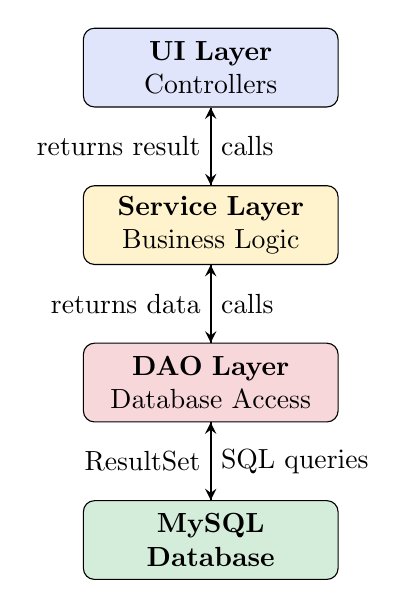
\begin{tikzpicture}[
    box/.style={rectangle, draw, fill=blue!20, text width=3cm, text centered, rounded corners, minimum height=1cm},
    arrow/.style={->, >=stealth, thick}
]
    \node[box, fill=purple!20] (ui) at (0,4) {\textbf{UI Layer}\\Controllers};
    \node[box, fill=yellow!20] (service) at (0,2) {\textbf{Service Layer}\\Business Logic};
    \node[box, fill=red!20] (dao) at (0,0) {\textbf{DAO Layer}\\Database Access};
    \node[box, fill=green!20] (db) at (0,-2) {\textbf{MySQL Database}};

    \draw[arrow] (ui) -- (service) node[midway, right] {calls};
    \draw[arrow] (service) -- (dao) node[midway, right] {calls};
    \draw[arrow] (dao) -- (db) node[midway, right] {SQL queries};
    \draw[arrow] (db) -- (dao) node[midway, left] {ResultSet};
    \draw[arrow] (dao) -- (service) node[midway, left] {returns data};
    \draw[arrow] (service) -- (ui) node[midway, left] {returns result};
\end{tikzpicture}
\end{center}

\subsection{Example Flow: User Login}

\textbf{Step 1:} User enters email + password and clicks ``Login''

\textbf{Step 2:} LoginController.onLogin() is called

\begin{lstlisting}
String token = authService.login(email, password);
\end{lstlisting}

\textbf{Step 3:} AuthService.login() validates credentials

\begin{lstlisting}
Optional<User> optUser = userDao.findByEmail(email);
if (optUser.isEmpty()) throw new Exception("User not found!");

User user = optUser.get();
if (!PasswordHasher.verify(password, user.getPasswordHash()))
    throw new Exception("Invalid password!");

return JwtService.issueToken(user.getId(), user.getRole());
\end{lstlisting}

\textbf{Step 4:} UserDao.findByEmail() queries the database

\begin{lstlisting}
Connection conn = DBConnection.getInstance();
PreparedStatement ps = conn.prepareStatement("SELECT * FROM users WHERE email=?");
ps.setString(1, email);
ResultSet rs = ps.executeQuery();

if (rs.next()) {
    return Optional.of(mapUser(rs));
}
\end{lstlisting}

\textbf{Step 5:} Database returns the user row → UserDao converts it to a User object → AuthService verifies the password → Generates a JWT token

\textbf{Step 6:} LoginController receives the token → Saves it to Session → Navigates to home screen

\begin{lstlisting}
Session.setToken(token);
HelloApplication.setRoot(new CustomerHomeController());
\end{lstlisting}

\begin{summarybox}
\textbf{In short:} User clicks button → Controller calls Service → Service calls DAO → DAO queries Database → Data flows back up the chain → UI updates!
\end{summarybox}

\newpage

% =====================================================
% STEP BY STEP RUN
% =====================================================
\section{👣 Full Step-By-Step Run (I Am The App!)}

\subsection{The Journey of a User}

\begin{tcolorbox}[colback=purple!10, colframe=purple!70!black, title=\textbf{🎬 Scene 1: App Startup}, fonttitle=\bfseries]
\textbf{Hi! I'm the ShopEase app! Let me show you my day...}

\textbf{8:00 AM:} Someone double-clicks my icon!

\textbf{8:00:01 AM:} Java calls my \texttt{main()} method in HelloApplication.java

\begin{lstlisting}
public static void main(String[] args) {
    launch();  // Starting up!
}
\end{lstlisting}

\textbf{8:00:02 AM:} JavaFX calls my \texttt{start()} method

\begin{lstlisting}
public void start(Stage stage) {
    mainStage = stage;
    setRoot(new LoginController());  // Show login screen
    stage.setTitle("E-Commerce App");
    stage.show();  // Ta-da! I'm visible!
}
\end{lstlisting}

\textbf{8:00:03 AM:} A window appears with a beautiful login screen! 🎮

I'm waiting patiently for someone to log in...
\end{tcolorbox}

\begin{tcolorbox}[colback=blue!10, colframe=blue!70!black, title=\textbf{🎬 Scene 2: User Logs In}, fonttitle=\bfseries]
\textbf{8:05 AM:} A user types their email and password and clicks ``Sign In''!

\textbf{Me (LoginController):} ``Okay, let me check that...''

\begin{lstlisting}
String email = emailField.getText().trim();  // "john@example.com"
String password = passwordField.getText().trim();  // "MyP@ss123"
\end{lstlisting}

\textbf{Me:} ``Hmm, looks good. Let me ask AuthService to verify this!''

\begin{lstlisting}
String token = authService.login(email, password);
\end{lstlisting}

\textbf{AuthService:} ``On it! Let me ask UserDao to find this user...''

\textbf{UserDao:} ``Checking the database... Found them! Here's the User object.''

\textbf{AuthService:} ``Great! Now let me verify the password...''

\begin{lstlisting}
if (!PasswordHasher.verify(password, user.getPasswordHash()))
    throw new Exception("Invalid password!");
\end{lstlisting}

\textbf{PasswordHasher:} ``Password matches! ✅''

\textbf{AuthService:} ``Awesome! Here's a JWT token for you!''

\begin{lstlisting}
return JwtService.issueToken(user.getId(), user.getRole());
\end{lstlisting}

\textbf{Me (LoginController):} ``Got the token! Saving it to Session...''

\begin{lstlisting}
Session.setToken(token);
\end{lstlisting}

\textbf{Me:} ``Now let me check if they're an admin or customer...''

\begin{lstlisting}
String role = JwtService.getRole(token);
if ("ADMIN".equals(role))
    HelloApplication.setRoot(new AdminProductsController());
else
    HelloApplication.setRoot(new CustomerHomeController());
\end{lstlisting}

\textbf{8:05:05 AM:} *WHOOSH* The screen changes to the Customer Home page!
\end{tcolorbox}

\begin{tcolorbox}[colback=green!10, colframe=green!70!black, title=\textbf{🎬 Scene 3: Browsing Products}, fonttitle=\bfseries]
\textbf{8:06 AM:} The CustomerHomeController appears!

\textbf{Me (CustomerHomeController):} ``Hello! Let me load all the products...''

\begin{lstlisting}
allProducts = productService.getAll();
\end{lstlisting}

\textbf{ProductService:} ``Asking ProductDao to fetch all products from the database...''

\textbf{ProductDao:} ``Running query: SELECT * FROM products...''

\textbf{Database:} ``Here are 150 products!''

\textbf{Me:} ``Great! I'll show them in a grid with product cards!''

\begin{lstlisting}
for (Product p : allProducts) {
    VBox card = createProductCard(p);
    productGrid.getChildren().add(card);
}
\end{lstlisting}

\textbf{User:} ``Wow, so many games! Let me filter by PS5...''

\textbf{Me:} ``On it!''

\begin{lstlisting}
filteredProducts = allProducts.stream()
    .filter(p -> p.getPlatforms().contains("PlayStation 5"))
    .collect(Collectors.toList());
\end{lstlisting}

\textbf{Me:} ``Here are 23 PS5 games!''
\end{tcolorbox}

\begin{tcolorbox}[colback=yellow!10, colframe=yellow!70!black, title=\textbf{🎬 Scene 4: Adding to Cart}, fonttitle=\bfseries]
\textbf{8:10 AM:} User clicks ``Add to Cart'' on Spider-Man 2!

\textbf{Me (CustomerHomeController):} ``Let me add that to the cart...''

\begin{lstlisting}
cartService.addItem(product, 1);
\end{lstlisting}

\textbf{CartService:} ``Okay, I'm adding Spider-Man 2 (quantity: 1) to the cart!''

\begin{lstlisting}
items.put(product, 1);
\end{lstlisting}

\textbf{Me:} ``Done! Showing a toast notification...''

\begin{lstlisting}
ToastNotification.success("Added to cart!");
\end{lstlisting}

\textbf{*A cute green notification slides in from the right*} ✅ Added to cart!

\textbf{User:} ``Awesome! Let me add a controller too...''

\textbf{Me:} ``Sure thing!''

*Repeats the process*

\textbf{CartService:} ``Now I have 2 items in the cart!''
\end{tcolorbox}

\begin{tcolorbox}[colback=red!10, colframe=red!70!black, title=\textbf{🎬 Scene 5: Viewing Cart \& Checkout}, fonttitle=\bfseries]
\textbf{8:12 AM:} User clicks the ``Cart'' button.

\textbf{Me (CustomerHomeController):} ``Navigating to cart...''

\begin{lstlisting}
HelloApplication.setRoot(new CartController());
\end{lstlisting}

\textbf{*Screen changes to CartController*}

\textbf{Me (CartController):} ``Loading cart items into a table...''

\begin{lstlisting}
for (Map.Entry<Product, Integer> e : cartService.getItems().entrySet()) {
    items.add(new CartItem(e.getKey(), e.getValue()));
}
cartTable.setItems(items);
\end{lstlisting}

\textbf{User sees:}
\begin{verbatim}
┌─────────────────────┬─────────┬──────────┬──────────┐
│ Product Name        │ Price   │ Quantity │ Subtotal │
├─────────────────────┼─────────┼──────────┼──────────┤
│ Spider-Man 2        │ $69.99  │ ×1       │ $69.99   │
│ DualSense Controller│ $59.99  │ ×1       │ $59.99   │
└─────────────────────┴─────────┴──────────┴──────────┘
Total: $129.98
\end{verbatim}

\textbf{User:} ``Looks good! Let me checkout!''

\textbf{*Clicks ``Proceed to Checkout''*}

\textbf{Me (CartController):} ``Navigating to checkout...''

\begin{lstlisting}
HelloApplication.setRoot(new CheckoutController());
\end{lstlisting}

\textbf{*Screen changes to CheckoutController*}

\textbf{Me (CheckoutController):} ``Alright! Let me show the shipping form and payment options...''

\textbf{User:} Enters shipping address and clicks ``Place Order''

\textbf{Me:} ``Creating the order!''

\begin{lstlisting}
int orderId = orderService.createOrder(userId, cartItems, shippingAddress);
\end{lstlisting}

\textbf{OrderService:} ``Saving the order to the database...''

\textbf{OrderDao:} ``INSERT INTO orders... Done! Order ID: 42''

\textbf{OrderService:} ``Now saving the order items...''

\textbf{OrderDao:} ``INSERT INTO order\_items... Done!''

\textbf{OrderService:} ``Clearing the cart...''

\textbf{CartService:} ``Cart is now empty!''

\textbf{Me (CheckoutController):} ``Success! Navigating to order confirmation...''

\textbf{*Shows success screen*} 🎉 Order placed successfully! Your order ID is \#42.
\end{tcolorbox}

\begin{tcolorbox}[colback=purple!10, colframe=purple!70!black, title=\textbf{🎬 Scene 6: Logout}, fonttitle=\bfseries]
\textbf{8:20 AM:} User clicks ``Logout''

\textbf{Me:} ``Clearing the session...''

\begin{lstlisting}
Session.clear();
\end{lstlisting}

\textbf{Session:} ``Token deleted! User is now logged out.''

\textbf{Me:} ``Navigating back to login screen...''

\begin{lstlisting}
HelloApplication.setRoot(new LoginController());
\end{lstlisting}

\textbf{*App returns to the login screen*}

\textbf{Me:} ``Thanks for shopping! See you next time! 👋''
\end{tcolorbox}

\newpage

% =====================================================
% WHAT I LEARNED
% =====================================================
\section{💡 What I Learned}

\begin{tcolorbox}[colback=green!10, colframe=green!70!black, title=\textbf{🎓 Key Takeaways}, fonttitle=\bfseries]

\subsection*{1. 🏗️ MVC Architecture}

I learned how to separate code into layers:
\begin{itemize}
    \item \textbf{Model} = Data (User, Product, Order)
    \item \textbf{View} = UI (Controllers that build screens)
    \item \textbf{Controller} = Logic (Services that coordinate everything)
\end{itemize}

This makes the code \textbf{organized} and \textbf{easy to maintain}!

\subsection*{2. 🔒 Security Matters}

I learned about:
\begin{itemize}
    \item \textbf{Password hashing} with bcrypt (never store plain passwords!)
    \item \textbf{JWT tokens} for authentication
    \item \textbf{Input validation} to prevent SQL injection
\end{itemize}

\subsection*{3. 🎨 Building UI Without FXML}

I learned how to create entire user interfaces using just Java code:
\begin{itemize}
    \item \textbf{VBox, HBox, BorderPane} for layouts
    \item \textbf{Inline CSS} for styling
    \item \textbf{Event handlers} for interactivity
\end{itemize}

\subsection*{4. 🗄️ Working with Databases}

I learned how to:
\begin{itemize}
    \item Connect to MySQL using JDBC
    \item Write SQL queries (SELECT, INSERT, UPDATE, DELETE)
    \item Map ResultSet rows to Java objects
    \item Use PreparedStatements to prevent SQL injection
\end{itemize}

\subsection*{5. 🛒 E-Commerce Logic}

I learned how online shopping works:
\begin{itemize}
    \item Shopping cart management
    \item Order processing
    \item Inventory tracking (stock management)
    \item Discounts and promotions
    \item Review systems
    \item Loyalty points
\end{itemize}

\subsection*{6. 🚀 Real-World Software Development}

I learned:
\begin{itemize}
    \item How to structure a large project
    \item How to use Maven for dependency management
    \item How to use Java Streams for filtering
    \item How to handle errors gracefully
    \item How to create reusable components
\end{itemize}

\end{tcolorbox}

\newpage

% =====================================================
% SCREENSHOTS
% =====================================================
\section{🖼️ Screenshot Placeholders}

\subsection*{📸 Login Screen}
\textbf{[Insert screenshot here]}

\textit{Description:} The beautiful purple gradient login screen with email and password fields.

\vspace{1cm}

\subsection*{📸 Customer Home - Product Grid}
\textbf{[Insert screenshot here]}

\textit{Description:} The main shopping page showing product cards in a grid layout with filters at the top.

\vspace{1cm}

\subsection*{📸 Product Details Popup}
\textbf{[Insert screenshot here]}

\textit{Description:} A popup showing detailed product information with Add to Cart and Wishlist buttons.

\vspace{1cm}

\subsection*{📸 Shopping Cart}
\textbf{[Insert screenshot here]}

\textit{Description:} The cart screen showing a table of items with quantities and total price.

\vspace{1cm}

\subsection*{📸 Checkout Screen}
\textbf{[Insert screenshot here]}

\textit{Description:} The checkout page with shipping address form and payment options.

\vspace{1cm}

\subsection*{📸 Admin Dashboard}
\textbf{[Insert screenshot here]}

\textit{Description:} The admin panel for managing products, orders, and reviews.

\vspace{1cm}

\subsection*{📸 Order History}
\textbf{[Insert screenshot here]}

\textit{Description:} A table showing the user's past orders with status tracking.

\vspace{1cm}

\subsection*{📸 Wishlist}
\textbf{[Insert screenshot here]}

\textit{Description:} The wishlist page showing saved favorite products.

\newpage

% =====================================================
% CONCLUSION
% =====================================================
\section*{🎉 Conclusion}

\begin{center}
\begin{tikzpicture}
    \draw[purple, ultra thick, rounded corners] (0,0) rectangle (12,4);
    \node[align=center, font=\Large\bfseries] at (6,2) {
        \textcolor{purple}{🎮 That's a wrap! 🎮} \\[0.5cm]
        This JavaFX e-commerce app is a complete, \\
        production-ready gaming store with: \\[0.3cm]
        ✅ Pure Java UI (no FXML) \\
        ✅ Secure authentication (JWT + bcrypt) \\
        ✅ MySQL database integration \\
        ✅ Beautiful, modern design \\
        ✅ Full shopping experience \\[0.3cm]
        \textcolor{green}{\textbf{Now go forth and build amazing things!}} 🚀
    };
\end{tikzpicture}
\end{center}

\vfill

\begin{center}
\textcolor{purple}{\textbf{\Large Made with ♥ and JavaFX}}

\textit{``Code is like humor. When you have to explain it, it's bad.'' – Cory House}
\end{center}

\end{document}
